\documentclass{beamer}
\usepackage[utf8]{inputenc}

\usetheme{Madrid}
\usecolortheme{default}
\usepackage{amsmath,amssymb,amsfonts,amsthm}
\usepackage{txfonts}
\usepackage{tkz-euclide}
\usepackage{listings}
\usepackage{adjustbox}
\usepackage{array}
\usepackage{tabularx}
\usepackage{gvv}
\usepackage{lmodern}
\usepackage{circuitikz}
\usepackage{tikz}
\usepackage{graphicx}

\setbeamertemplate{page number in head/foot}[totalframenumber]

\usepackage{tcolorbox}
\tcbuselibrary{minted,breakable,xparse,skins}



\definecolor{bg}{gray}{0.95}
\DeclareTCBListing{mintedbox}{O{}m!O{}}{%
  breakable=true,
  listing engine=minted,
  listing only,
  minted language=#2,
  minted style=default,
  minted options={%
    linenos,
    gobble=0,
    breaklines=true,
    breakafter=,,
    fontsize=\small,
    numbersep=8pt,
    #1},
  boxsep=0pt,
  left skip=0pt,
  right skip=0pt,
  left=25pt,
  right=0pt,
  top=3pt,
  bottom=3pt,
  arc=5pt,
  leftrule=0pt,
  rightrule=0pt,
  bottomrule=2pt,
  toprule=2pt,
  colback=bg,
  colframe=orange!70,
  enhanced,
  overlay={%
    \begin{tcbclipinterior}
    \fill[orange!20!white] (frame.south west) rectangle ([xshift=20pt]frame.north west);
    \end{tcbclipinterior}},
  #3,
}
\lstset{
    language=C,
    basicstyle=\ttfamily\small,
    keywordstyle=\color{blue},
    stringstyle=\color{orange},
    commentstyle=\color{green!60!black},
    numbers=left,
    numberstyle=\tiny\color{gray},
    breaklines=true,
    showstringspaces=false,
}
%------------------------------------------------------------

\title
{9.8.5}
\date{September 22, 2025}
\author 
{AI25BTECH11003 - Bhavesh Gaikwad}



\begin{document}


\frame{\titlepage}
\begin{frame}{Question}
Let $\vec{S}$ be the focus of the parabola $y^2 = 8x$ and let PQ be the common chord of the circle $x^2 + y^2 - 2x - 4y = 0$ and the given parabola. The area of the triangle PQS is
\end{frame}


\begin{frame}[fragile]
    \frametitle{Theoretical Solution}
      Given:\\
$\quad \text{Circle: }x^2 + y^2 - 2x - 4y = 0$\\
$\text{Parabola: }y^2 = 8x$\\\\


Parameters of the Circle:
\begin{equation}
\vec{V}_1 = \myvec{1 & 0 \\ 0 & 1}, \, \vec{u}_1 = \myvec{-1 \\ -2}, \, f_1 = 0   
\end{equation}

Parameters of the Parabola:
\begin{equation}
\vec{V}_2 = \myvec{0 & 0 \\ 0 & 1}, \, \vec{u}_2 = \myvec{-4 \\ 0}, \, f_2 = 0, \, \vec{S} = \myvec{2e \\ 0 } = \myvec{2 \\ 0}   
\end{equation}

Points of Intersection of Circle and Parabola can be given as:
\begin{equation}
\vec{X}^\top(\vec{V}_1+\mu\vec{V}_2)\vec{X} + 2(\vec{u}_1+\mu\vec{u}_2)^\top\vec{X} + (f_1 + \mu f_2) = 0
\end{equation}
\end{frame}


\begin{frame}[fragile]
    \frametitle{Theoretical Solution}
\begin{equation}
\vec{X}^\top\myvec{1 & 0 \\ 0 & 1+\mu}\vec{X} - 2\myvec{1+4\mu & 2}\vec{X} = 0    
\end{equation}

To degenerate a conic into a line, we can find values of $\mu$ by
\begin{equation}
\norm{\vec{M}_1 + \mu\vec{M}_2} =0
\end{equation}
where $\vec{M}_i = \myvec{\vec{V}_i & \vec{u}_i \\ \vec{u}_i^\top & f_i}$\\

From Equation 5, we get 
\begin{equation}
    (4\mu+1)^2(\mu + 1) = -4
\end{equation}

\begin{equation}
\Rightarrow \, \, \mu = \dfrac{-5}{4} \text{ (as the only real solution.)}    
\end{equation}
\end{frame}

\begin{frame}[fragile]
\frametitle{Theoretical Solution}
 Substituting the value of $\mu$ in Equation 4,
\begin{equation}
\vec{X}^\top\myvec{1 & 0 \\ 0 & -1/4}\vec{X} + \myvec{8 & -4}\vec{X} = 0
\end{equation}

\begin{equation}
    (2x+y+16)(2x-y) = 0
\end{equation}

\begin{equation}
   \Rightarrow \, \, 2x + y + 16 =0 \text{ OR } 2x-y=0
\end{equation}

From Line $2x + y + 16 =0$, we get no points of intersection with both the conics.\\
Thus, Rejected this Case.\\

From Line $2x-y=0$
\begin{equation}
    \vec{X} = k\myvec{2 \\ -1} 
\end{equation}
\end{frame}

\begin{frame}[fragile]
\frametitle{Theoretical Solution}
 The Intersection of the given conic with the given line can be written as:
\begin{equation}
    \vec{x}_j = \vec{h} + k_j\vec{m}
\end{equation}

\begin{equation}
where, \, \vec{h} = \myvec{0 \\ 0} \, \& \, \vec{m} = \myvec{2 \\ -1}   
\end{equation}

\begin{equation}
    k_{j} = \left( \dfrac{1}{\vec{m}^\top\vec{V}_i\vec{m}} \right) \left( 
    -\vec{m}^\top(\vec{V}_i\vec{h}+\vec{u}_i) \, \pm \, \sqrt{[\vec{m}^\top(\vec{V}_i\vec{h}+\vec{u}_i)]^2 - g(h)(\vec{m}^\top\vec{V}_i\vec{m})} \right) 
\end{equation}

After Solving the Equation 12 with circle and parabola, We get common points of intersection as:
\begin{equation}
    \vec{X}_1 = \myvec{0 \\ 0} \qquad \& \qquad \vec{X}_2 = \myvec{2 \\ 4}
\end{equation}
\end{frame}

\begin{frame}[fragile]
\frametitle{Theoretical Solution}
 
Therefore,
Let $\vec{P} = \myvec{0 \\ 0}$ and $\vec{Q} = \myvec{2 \\ 4}$\\\\

The Area of Triangle PQS is:
\begin{equation}
    Area(\triangle PQS) = \dfrac{1}{2}\norm{\vec{SP} \times \vec{QP}} = 4
\end{equation}

\begin{align*}
    \boxed{\text{The Area of $\triangle PQS$ is 4 sq.units.}}
\end{align*}
\end{frame}


\begin{frame}{Intersection of Two Conics and Triangle PQS}
\begin{figure}
   \centering
    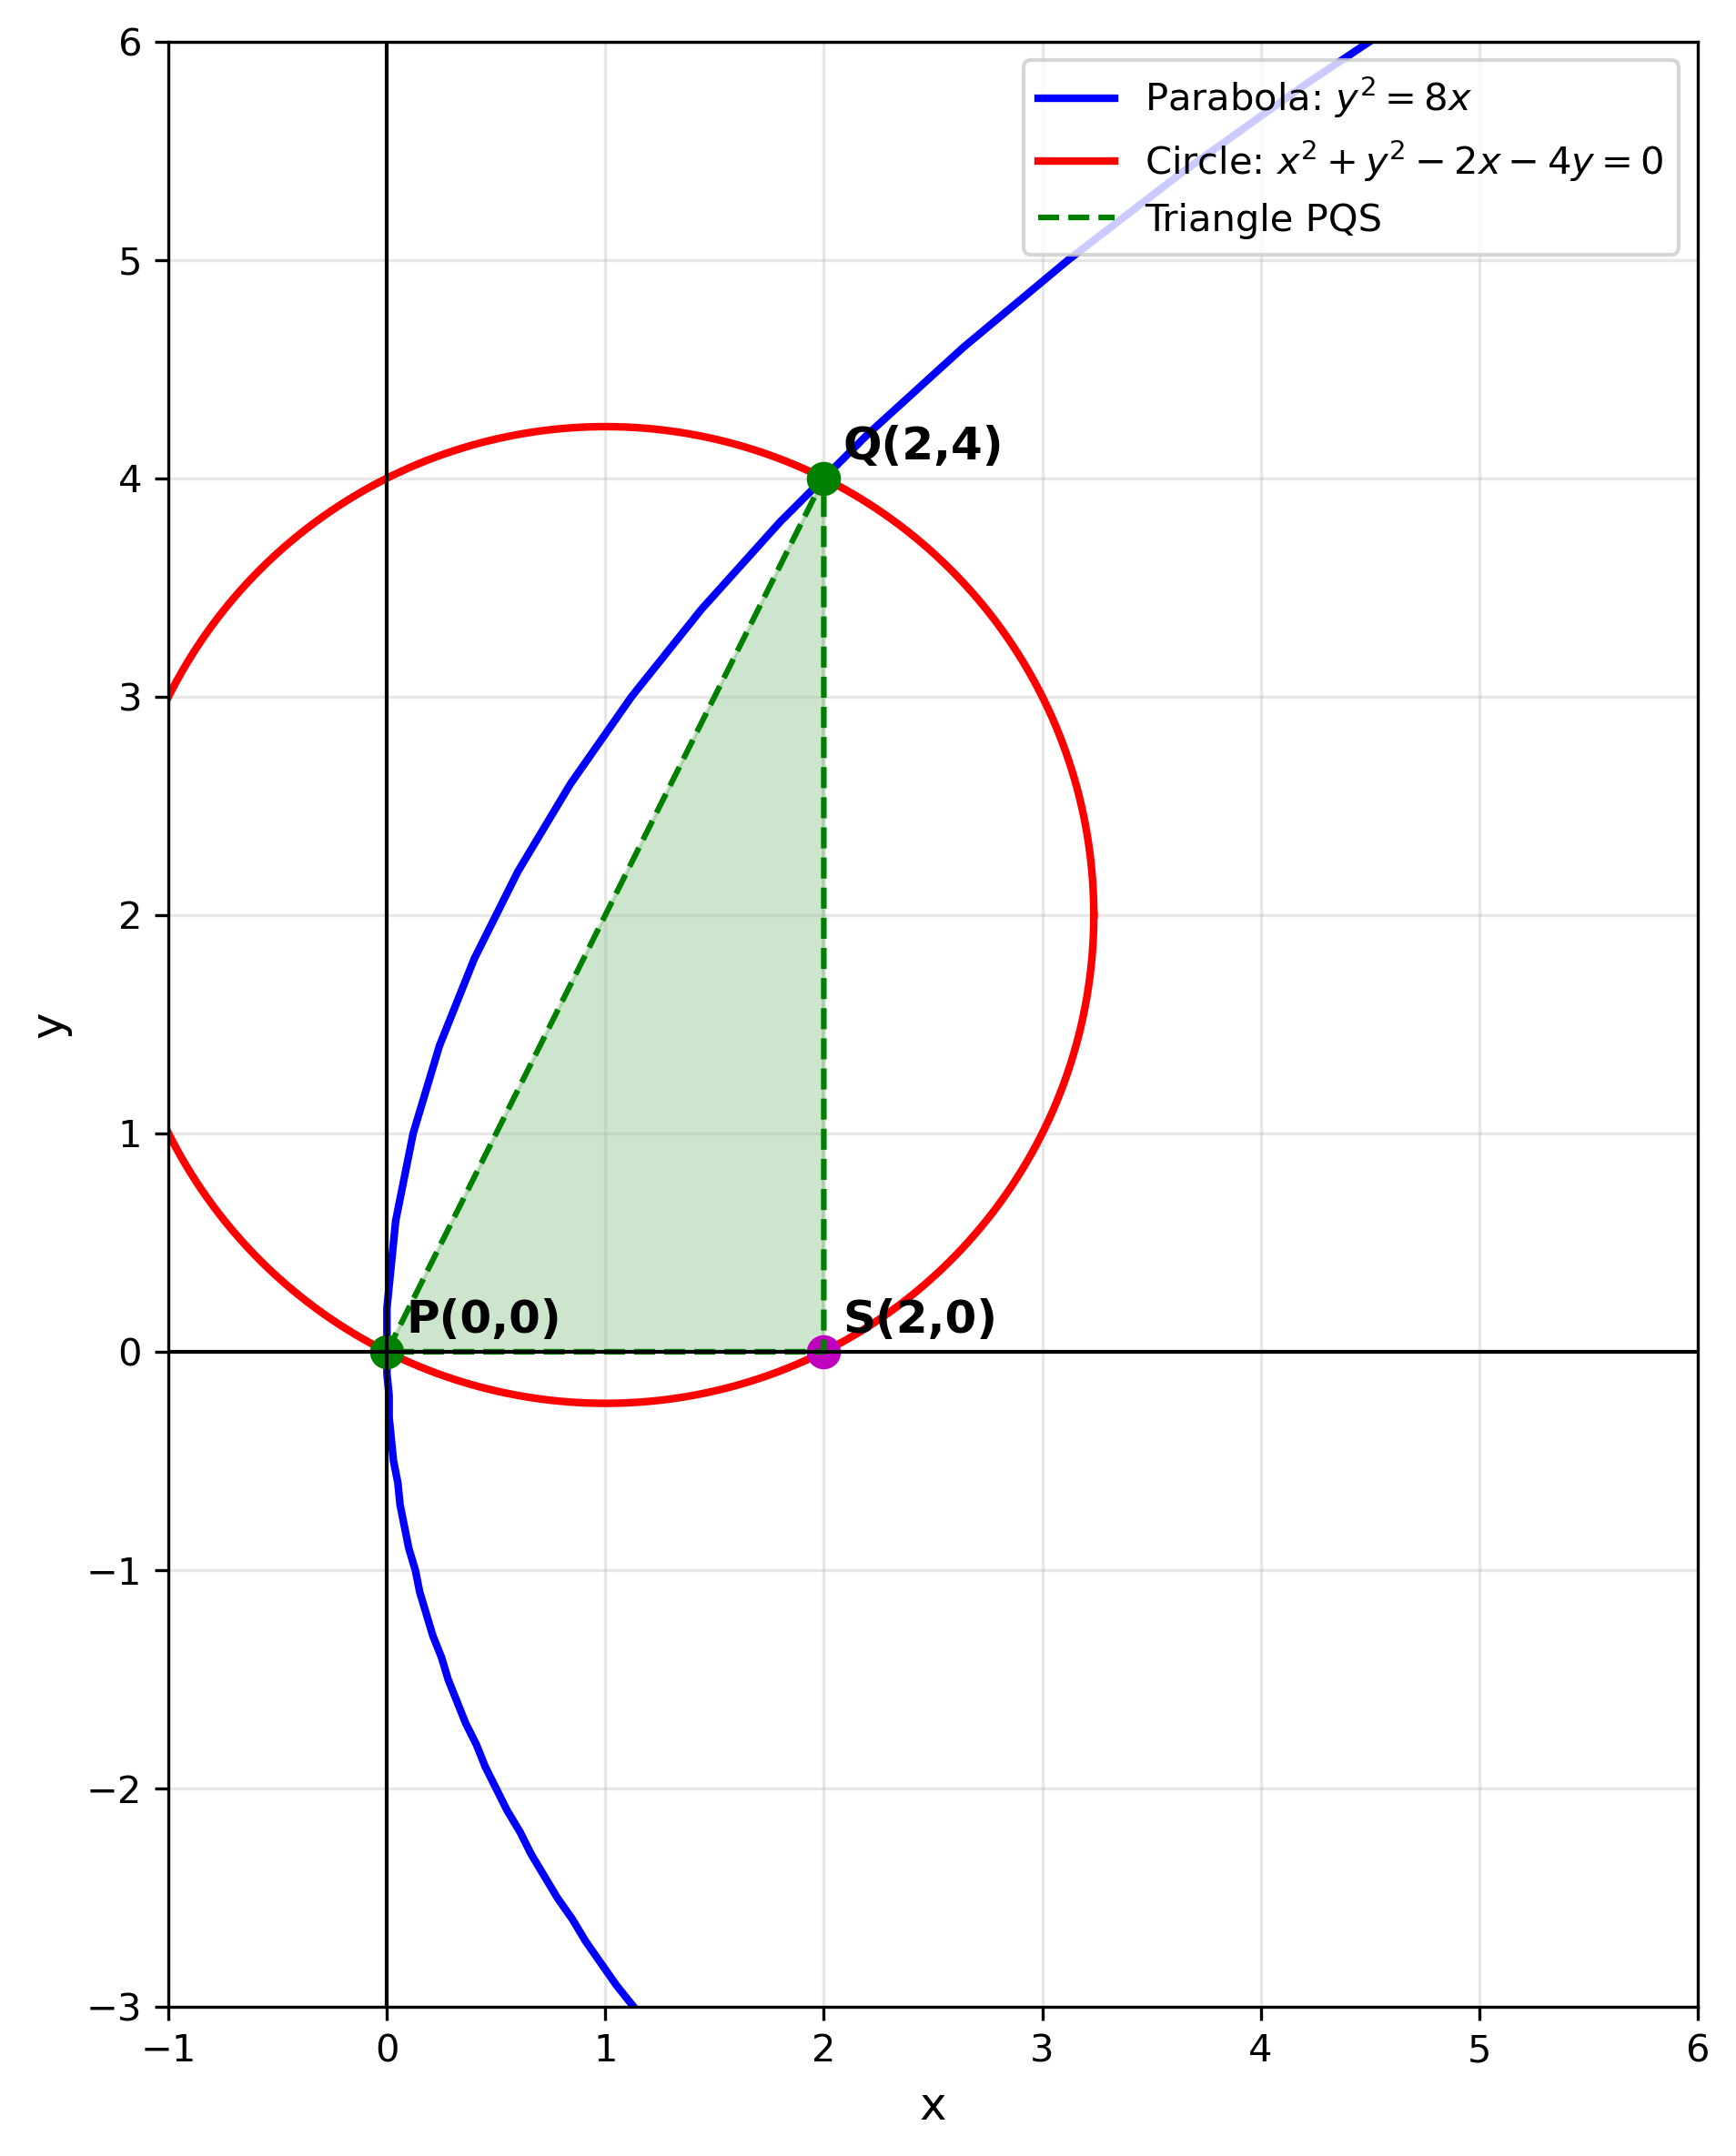
\includegraphics[width=\columnwidth, height=0.8\textheight, keepaspectratio]{figs/fig1.png}
    \label{fig:Beamer/figs/fig1.png}
\end{figure}
\end{frame}

\end{document}